
\documentclass[11pt,compress,t,notes=noshow, xcolor=table]{beamer}
\usepackage[]{graphicx}\usepackage[]{color}
% maxwidth is the original width if it is less than linewidth
% otherwise use linewidth (to make sure the graphics do not exceed the margin)
\makeatletter
\def\maxwidth{ %
  \ifdim\Gin@nat@width>\linewidth
    \linewidth
  \else
    \Gin@nat@width
  \fi
}
\makeatother

\definecolor{fgcolor}{rgb}{0.345, 0.345, 0.345}
\newcommand{\hlnum}[1]{\textcolor[rgb]{0.686,0.059,0.569}{#1}}%
\newcommand{\hlstr}[1]{\textcolor[rgb]{0.192,0.494,0.8}{#1}}%
\newcommand{\hlcom}[1]{\textcolor[rgb]{0.678,0.584,0.686}{\textit{#1}}}%
\newcommand{\hlopt}[1]{\textcolor[rgb]{0,0,0}{#1}}%
\newcommand{\hlstd}[1]{\textcolor[rgb]{0.345,0.345,0.345}{#1}}%
\newcommand{\hlkwa}[1]{\textcolor[rgb]{0.161,0.373,0.58}{\textbf{#1}}}%
\newcommand{\hlkwb}[1]{\textcolor[rgb]{0.69,0.353,0.396}{#1}}%
\newcommand{\hlkwc}[1]{\textcolor[rgb]{0.333,0.667,0.333}{#1}}%
\newcommand{\hlkwd}[1]{\textcolor[rgb]{0.737,0.353,0.396}{\textbf{#1}}}%
\let\hlipl\hlkwb

\usepackage{framed}
\makeatletter
\newenvironment{kframe}{%
 \def\at@end@of@kframe{}%
 \ifinner\ifhmode%
  \def\at@end@of@kframe{\end{minipage}}%
  \begin{minipage}{\columnwidth}%
 \fi\fi%
 \def\FrameCommand##1{\hskip\@totalleftmargin \hskip-\fboxsep
 \colorbox{shadecolor}{##1}\hskip-\fboxsep
     % There is no \\@totalrightmargin, so:
     \hskip-\linewidth \hskip-\@totalleftmargin \hskip\columnwidth}%
 \MakeFramed {\advance\hsize-\width
   \@totalleftmargin\z@ \linewidth\hsize
   \@setminipage}}%
 {\par\unskip\endMakeFramed%
 \at@end@of@kframe}
\makeatother

\definecolor{shadecolor}{rgb}{.97, .97, .97}
\definecolor{messagecolor}{rgb}{0, 0, 0}
\definecolor{warningcolor}{rgb}{1, 0, 1}
\definecolor{errorcolor}{rgb}{1, 0, 0}
\newenvironment{knitrout}{}{} % an empty environment to be redefined in TeX

\usepackage{alltt}
\newcommand{\SweaveOpts}[1]{}  % do not interfere with LaTeX
\newcommand{\SweaveInput}[1]{} % because they are not real TeX commands
\newcommand{\Sexpr}[1]{}       % will only be parsed by R
\newcommand{\xmark}{\ding{55}}%


\usepackage[english]{babel}
\usepackage[utf8]{inputenc}

\usepackage{dsfont}
\usepackage{verbatim}
\usepackage{amsmath}
\usepackage{amsfonts}
\usepackage{amssymb}
\usepackage{bm}
\usepackage{csquotes}
\usepackage{multirow}
\usepackage{longtable}
\usepackage{booktabs}
\usepackage{enumerate}
\usepackage[absolute,overlay]{textpos}
\usepackage{psfrag}
\usepackage{algorithm}
\usepackage{algpseudocode}
\usepackage{eqnarray}
\usepackage{arydshln}
\usepackage{tabularx}
\usepackage{placeins}
\usepackage{tikz}
\usepackage{setspace}
\usepackage{colortbl}
\usepackage{mathtools}
\usepackage{wrapfig}
\usepackage{bm}
\usepackage{amsmath}
\usepackage{pifont}

\usetikzlibrary{shapes,arrows,automata,positioning,calc,chains,trees, shadows}
\tikzset{
  %Define standard arrow tip
  >=stealth',
  %Define style for boxes
  punkt/.style={
    rectangle,
    rounded corners,
    draw=black, very thick,
    text width=6.5em,
    minimum height=2em,
    text centered},
  % Define arrow style
  pil/.style={
    ->,
    thick,
    shorten <=2pt,
    shorten >=2pt,}
}

\usepackage{subfig}

% Defines macros and environments
\usepackage{../../style/lmu-lecture}


\let\code=\texttt
\let\proglang=\textsf

\setkeys{Gin}{width=0.9\textwidth}

\setbeamertemplate{frametitle}{\expandafter\uppercase\expandafter\insertframetitle}

\usepackage{bbm}
% basic latex stuff
\newcommand{\pkg}[1]{{\fontseries{b}\selectfont #1}} %fontstyle for R packages
\newcommand{\lz}{\vspace{0.5cm}} %vertical space
\newcommand{\dlz}{\vspace{1cm}} %double vertical space
\newcommand{\oneliner}[1] % Oneliner for important statements
{\begin{block}{}\begin{center}\begin{Large}#1\end{Large}\end{center}\end{block}}


%new environments
\newenvironment{vbframe}  %frame with breaks and verbatim
{
 \begin{frame}[containsverbatim,allowframebreaks]
}
{
\end{frame}
}

\newenvironment{vframe}  %frame with verbatim without breaks (to avoid numbering one slided frames)
{
 \begin{frame}[containsverbatim]
}
{
\end{frame}
}

\newenvironment{blocki}[1]   % itemize block
{
 \begin{block}{#1}\begin{itemize}
}
{
\end{itemize}\end{block}
}

\newenvironment{fragileframe}[2]{  %fragile frame with framebreaks
\begin{frame}[allowframebreaks, fragile, environment = fragileframe]
\frametitle{#1}
#2}
{\end{frame}}


\newcommand{\myframe}[2]{  %short for frame with framebreaks
\begin{frame}[allowframebreaks]
\frametitle{#1}
#2
\end{frame}}

\newcommand{\remark}[1]{
  \textbf{Remark:} #1
}


\newenvironment{deleteframe}
{
\begingroup
\usebackgroundtemplate{
\includegraphics[width=\paperwidth,height=\paperheight]{../style/color/red.png}}
 \begin{frame}
}
{
\end{frame}
\endgroup
}
\newenvironment{simplifyframe}
{
\begingroup
\usebackgroundtemplate{
\includegraphics[width=\paperwidth,height=\paperheight]{../style/color/yellow.png}}
 \begin{frame}
}
{
\end{frame}
\endgroup
}\newenvironment{draftframe}
{
\begingroup
\usebackgroundtemplate{
\includegraphics[width=\paperwidth,height=\paperheight]{../style/color/green.jpg}}
 \begin{frame}
}
{
\end{frame}
\endgroup
}
% https://tex.stackexchange.com/a/261480: textcolor that works in mathmode
\makeatletter
\renewcommand*{\@textcolor}[3]{%
  \protect\leavevmode
  \begingroup
    \color#1{#2}#3%
  \endgroup
}
\makeatother





% math spaces
\ifdefined\N                                                                
\renewcommand{\N}{\mathds{N}} % N, naturals
\else \newcommand{\N}{\mathds{N}} \fi 
\newcommand{\Z}{\mathds{Z}} % Z, integers
\newcommand{\Q}{\mathds{Q}} % Q, rationals
\newcommand{\R}{\mathds{R}} % R, reals
\ifdefined\C 
  \renewcommand{\C}{\mathds{C}} % C, complex
\else \newcommand{\C}{\mathds{C}} \fi
\newcommand{\continuous}{\mathcal{C}} % C, space of continuous functions
\newcommand{\M}{\mathcal{M}} % machine numbers
\newcommand{\epsm}{\epsilon_m} % maximum error

% counting / finite sets
\newcommand{\setzo}{\{0, 1\}} % set 0, 1
\newcommand{\setmp}{\{-1, +1\}} % set -1, 1
\newcommand{\unitint}{[0, 1]} % unit interval

% basic math stuff
\newcommand{\xt}{\tilde x} % x tilde
\newcommand{\argmax}{\operatorname{arg\,max}} % argmax
\newcommand{\argmin}{\operatorname{arg\,min}} % argmin
\newcommand{\argminlim}{\mathop{\mathrm{arg\,min}}\limits} % argmax with limits
\newcommand{\argmaxlim}{\mathop{\mathrm{arg\,max}}\limits} % argmin with limits  
\newcommand{\sign}{\operatorname{sign}} % sign, signum
\newcommand{\I}{\mathbb{I}} % I, indicator
\newcommand{\order}{\mathcal{O}} % O, order
\newcommand{\pd}[2]{\frac{\partial{#1}}{\partial #2}} % partial derivative
\newcommand{\floorlr}[1]{\left\lfloor #1 \right\rfloor} % floor
\newcommand{\ceillr}[1]{\left\lceil #1 \right\rceil} % ceiling

% sums and products
\newcommand{\sumin}{\sum\limits_{i=1}^n} % summation from i=1 to n
\newcommand{\sumim}{\sum\limits_{i=1}^m} % summation from i=1 to m
\newcommand{\sumjn}{\sum\limits_{j=1}^n} % summation from j=1 to p
\newcommand{\sumjp}{\sum\limits_{j=1}^p} % summation from j=1 to p
\newcommand{\sumik}{\sum\limits_{i=1}^k} % summation from i=1 to k
\newcommand{\sumkg}{\sum\limits_{k=1}^g} % summation from k=1 to g
\newcommand{\sumjg}{\sum\limits_{j=1}^g} % summation from j=1 to g
\newcommand{\meanin}{\frac{1}{n} \sum\limits_{i=1}^n} % mean from i=1 to n
\newcommand{\meanim}{\frac{1}{m} \sum\limits_{i=1}^m} % mean from i=1 to n
\newcommand{\meankg}{\frac{1}{g} \sum\limits_{k=1}^g} % mean from k=1 to g
\newcommand{\prodin}{\prod\limits_{i=1}^n} % product from i=1 to n
\newcommand{\prodkg}{\prod\limits_{k=1}^g} % product from k=1 to g
\newcommand{\prodjp}{\prod\limits_{j=1}^p} % product from j=1 to p

% linear algebra
\newcommand{\one}{\boldsymbol{1}} % 1, unitvector
\newcommand{\zero}{\mathbf{0}} % 0-vector
\newcommand{\id}{\boldsymbol{I}} % I, identity
\newcommand{\diag}{\operatorname{diag}} % diag, diagonal
\newcommand{\trace}{\operatorname{tr}} % tr, trace
\newcommand{\spn}{\operatorname{span}} % span
\newcommand{\scp}[2]{\left\langle #1, #2 \right\rangle} % <.,.>, scalarproduct
\newcommand{\mat}[1]{\begin{pmatrix} #1 \end{pmatrix}} % short pmatrix command
\newcommand{\Amat}{\mathbf{A}} % matrix A
\newcommand{\Deltab}{\mathbf{\Delta}} % error term for vectors

% basic probability + stats
\renewcommand{\P}{\mathds{P}} % P, probability
\newcommand{\E}{\mathds{E}} % E, expectation
\newcommand{\var}{\mathsf{Var}} % Var, variance
\newcommand{\cov}{\mathsf{Cov}} % Cov, covariance
\newcommand{\corr}{\mathsf{Corr}} % Corr, correlation
\newcommand{\normal}{\mathcal{N}} % N of the normal distribution
\newcommand{\iid}{\overset{i.i.d}{\sim}} % dist with i.i.d superscript
\newcommand{\distas}[1]{\overset{#1}{\sim}} % ... is distributed as ...

% machine learning
\newcommand{\Xspace}{\mathcal{X}} % X, input space
\newcommand{\Yspace}{\mathcal{Y}} % Y, output space
\newcommand{\nset}{\{1, \ldots, n\}} % set from 1 to n
\newcommand{\pset}{\{1, \ldots, p\}} % set from 1 to p
\newcommand{\gset}{\{1, \ldots, g\}} % set from 1 to g
\newcommand{\Pxy}{\mathbb{P}_{xy}} % P_xy
\newcommand{\Exy}{\mathbb{E}_{xy}} % E_xy: Expectation over random variables xy
\newcommand{\xv}{\mathbf{x}} % vector x (bold)
\newcommand{\xtil}{\tilde{\mathbf{x}}} % vector x-tilde (bold)
\newcommand{\yv}{\mathbf{y}} % vector y (bold)
\newcommand{\xy}{(\xv, y)} % observation (x, y)
\newcommand{\xvec}{\left(x_1, \ldots, x_p\right)^\top} % (x1, ..., xp) 
\newcommand{\Xmat}{\mathbf{X}} % Design matrix
\newcommand{\allDatasets}{\mathds{D}} % The set of all datasets
\newcommand{\allDatasetsn}{\mathds{D}_n}  % The set of all datasets of size n 
\newcommand{\D}{\mathcal{D}} % D, data
\newcommand{\Dn}{\D_n} % D_n, data of size n
\newcommand{\Dtrain}{\mathcal{D}_{\text{train}}} % D_train, training set
\newcommand{\Dtest}{\mathcal{D}_{\text{test}}} % D_test, test set
\newcommand{\xyi}[1][i]{\left(\xv^{(#1)}, y^{(#1)}\right)} % (x^i, y^i), i-th observation
\newcommand{\Dset}{\left( \xyi[1], \ldots, \xyi[n]\right)} % {(x1,y1)), ..., (xn,yn)}, data
\newcommand{\defAllDatasetsn}{(\Xspace \times \Yspace)^n} % Def. of the set of all datasets of size n 
\newcommand{\defAllDatasets}{\bigcup_{n \in \N}(\Xspace \times \Yspace)^n} % Def. of the set of all datasets 
\newcommand{\xdat}{\left\{ \xv^{(1)}, \ldots, \xv^{(n)}\right\}} % {x1, ..., xn}, input data
\newcommand{\ydat}{\left\{ \yv^{(1)}, \ldots, \yv^{(n)}\right\}} % {y1, ..., yn}, input data
\newcommand{\yvec}{\left(y^{(1)}, \hdots, y^{(n)}\right)^\top} % (y1, ..., yn), vector of outcomes
\renewcommand{\xi}[1][i]{\xv^{(#1)}} % x^i, i-th observed value of x
\newcommand{\yi}[1][i]{y^{(#1)}} % y^i, i-th observed value of y 
\newcommand{\xivec}{\left(x^{(i)}_1, \ldots, x^{(i)}_p\right)^\top} % (x1^i, ..., xp^i), i-th observation vector
\newcommand{\xj}{\xv_j} % x_j, j-th feature
\newcommand{\xjvec}{\left(x^{(1)}_j, \ldots, x^{(n)}_j\right)^\top} % (x^1_j, ..., x^n_j), j-th feature vector
\newcommand{\phiv}{\mathbf{\phi}} % Basis transformation function phi
\newcommand{\phixi}{\mathbf{\phi}^{(i)}} % Basis transformation of xi: phi^i := phi(xi)

%%%%%% ml - models general
\newcommand{\lamv}{\bm{\lambda}} % lambda vector, hyperconfiguration vector
\newcommand{\Lam}{\bm{\Lambda}}	 % Lambda, space of all hpos
% Inducer / Inducing algorithm
\newcommand{\preimageInducer}{\left(\defAllDatasets\right)\times\Lam} % Set of all datasets times the hyperparameter space
\newcommand{\preimageInducerShort}{\allDatasets\times\Lam} % Set of all datasets times the hyperparameter space
% Inducer / Inducing algorithm
\newcommand{\ind}{\mathcal{I}} % Inducer, inducing algorithm, learning algorithm 

% continuous prediction function f
\newcommand{\ftrue}{f_{\text{true}}}  % True underlying function (if a statistical model is assumed)
\newcommand{\ftruex}{\ftrue(\xv)} % True underlying function (if a statistical model is assumed)
\newcommand{\fx}{f(\xv)} % f(x), continuous prediction function
\newcommand{\fdomains}{f: \Xspace \rightarrow \R^g} % f with domain and co-domain
\newcommand{\Hspace}{\mathcal{H}} % hypothesis space where f is from
\newcommand{\fbayes}{f^{\ast}} % Bayes-optimal model
\newcommand{\fxbayes}{f^{\ast}(\xv)} % Bayes-optimal model
\newcommand{\fkx}[1][k]{f_{#1}(\xv)} % f_j(x), discriminant component function
\newcommand{\fh}{\hat{f}} % f hat, estimated prediction function
\newcommand{\fxh}{\fh(\xv)} % fhat(x)
\newcommand{\fxt}{f(\xv ~|~ \thetab)} % f(x | theta)
\newcommand{\fxi}{f\left(\xv^{(i)}\right)} % f(x^(i))
\newcommand{\fxih}{\hat{f}\left(\xv^{(i)}\right)} % f(x^(i))
\newcommand{\fxit}{f\left(\xv^{(i)} ~|~ \thetab\right)} % f(x^(i) | theta)
\newcommand{\fhD}{\fh_{\D}} % fhat_D, estimate of f based on D
\newcommand{\fhDtrain}{\fh_{\Dtrain}} % fhat_Dtrain, estimate of f based on D
\newcommand{\fhDnlam}{\fh_{\Dn, \lamv}} %model learned on Dn with hp lambda
\newcommand{\fhDlam}{\fh_{\D, \lamv}} %model learned on D with hp lambda
\newcommand{\fhDnlams}{\fh_{\Dn, \lamv^\ast}} %model learned on Dn with optimal hp lambda 
\newcommand{\fhDlams}{\fh_{\D, \lamv^\ast}} %model learned on D with optimal hp lambda 

% discrete prediction function h
\newcommand{\hx}{h(\xv)} % h(x), discrete prediction function
\newcommand{\hh}{\hat{h}} % h hat
\newcommand{\hxh}{\hat{h}(\xv)} % hhat(x)
\newcommand{\hxt}{h(\xv | \thetab)} % h(x | theta)
\newcommand{\hxi}{h\left(\xi\right)} % h(x^(i))
\newcommand{\hxit}{h\left(\xi ~|~ \thetab\right)} % h(x^(i) | theta)
\newcommand{\hbayes}{h^{\ast}} % Bayes-optimal classification model
\newcommand{\hxbayes}{h^{\ast}(\xv)} % Bayes-optimal classification model

% yhat
\newcommand{\yh}{\hat{y}} % yhat for prediction of target
\newcommand{\yih}{\hat{y}^{(i)}} % yhat^(i) for prediction of ith targiet
\newcommand{\resi}{\yi- \yih}

% theta
\newcommand{\thetah}{\hat{\theta}} % theta hat
\newcommand{\thetab}{\bm{\theta}} % theta vector
\newcommand{\thetabh}{\bm{\hat\theta}} % theta vector hat
\newcommand{\thetat}[1][t]{\thetab^{[#1]}} % theta^[t] in optimization
\newcommand{\thetatn}[1][t]{\thetab^{[#1 +1]}} % theta^[t+1] in optimization
\newcommand{\thetahDnlam}{\thetabh_{\Dn, \lamv}} %theta learned on Dn with hp lambda
\newcommand{\thetahDlam}{\thetabh_{\D, \lamv}} %theta learned on D with hp lambda
\newcommand{\mint}{\min_{\thetab \in \Theta}} % min problem theta
\newcommand{\argmint}{\argmin_{\thetab \in \Theta}} % argmin theta

% densities + probabilities
% pdf of x 
\newcommand{\pdf}{p} % p
\newcommand{\pdfx}{p(\xv)} % p(x)
\newcommand{\pixt}{\pi(\xv~|~ \thetab)} % pi(x|theta), pdf of x given theta
\newcommand{\pixit}[1][i]{\pi\left(\xi[#1] ~|~ \thetab\right)} % pi(x^i|theta), pdf of x given theta
\newcommand{\pixii}[1][i]{\pi\left(\xi[#1]\right)} % pi(x^i), pdf of i-th x 

% pdf of (x, y)
\newcommand{\pdfxy}{p(\xv,y)} % p(x, y)
\newcommand{\pdfxyt}{p(\xv, y ~|~ \thetab)} % p(x, y | theta)
\newcommand{\pdfxyit}{p\left(\xi, \yi ~|~ \thetab\right)} % p(x^(i), y^(i) | theta)

% pdf of x given y
\newcommand{\pdfxyk}[1][k]{p(\xv | y= #1)} % p(x | y = k)
\newcommand{\lpdfxyk}[1][k]{\log p(\xv | y= #1)} % log p(x | y = k)
\newcommand{\pdfxiyk}[1][k]{p\left(\xi | y= #1 \right)} % p(x^i | y = k)

% prior probabilities
\newcommand{\pik}[1][k]{\pi_{#1}} % pi_k, prior
\newcommand{\lpik}[1][k]{\log \pi_{#1}} % log pi_k, log of the prior
\newcommand{\pit}{\pi(\thetab)} % Prior probability of parameter theta

% posterior probabilities
\newcommand{\post}{\P(y = 1 ~|~ \xv)} % P(y = 1 | x), post. prob for y=1
\newcommand{\postk}[1][k]{\P(y = #1 ~|~ \xv)} % P(y = k | y), post. prob for y=k
\newcommand{\pidomains}{\pi: \Xspace \rightarrow \unitint} % pi with domain and co-domain
\newcommand{\pibayes}{\pi^{\ast}} % Bayes-optimal classification model
\newcommand{\pixbayes}{\pi^{\ast}(\xv)} % Bayes-optimal classification model
\newcommand{\pix}{\pi(\xv)} % pi(x), P(y = 1 | x)
\newcommand{\piv}{\bm{\pi}} % pi, bold, as vector
\newcommand{\pikx}[1][k]{\pi_{#1}(\xv)} % pi_k(x), P(y = k | x)
\newcommand{\pikxt}[1][k]{\pi_{#1}(\xv ~|~ \thetab)} % pi_k(x | theta), P(y = k | x, theta)
\newcommand{\pixh}{\hat \pi(\xv)} % pi(x) hat, P(y = 1 | x) hat
\newcommand{\pikxh}[1][k]{\hat \pi_{#1}(\xv)} % pi_k(x) hat, P(y = k | x) hat
\newcommand{\pixih}{\hat \pi(\xi)} % pi(x^(i)) with hat
\newcommand{\pikxih}[1][k]{\hat \pi_{#1}(\xi)} % pi_k(x^(i)) with hat
\newcommand{\pdfygxt}{p(y ~|~\xv, \thetab)} % p(y | x, theta)
\newcommand{\pdfyigxit}{p\left(\yi ~|~\xi, \thetab\right)} % p(y^i |x^i, theta)
\newcommand{\lpdfygxt}{\log \pdfygxt } % log p(y | x, theta)
\newcommand{\lpdfyigxit}{\log \pdfyigxit} % log p(y^i |x^i, theta)

% probababilistic
\newcommand{\bayesrulek}[1][k]{\frac{\P(\xv | y= #1) \P(y= #1)}{\P(\xv)}} % Bayes rule
\newcommand{\muk}{\bm{\mu_k}} % mean vector of class-k Gaussian (discr analysis) 

% residual and margin
\newcommand{\eps}{\epsilon} % residual, stochastic
\newcommand{\epsi}{\epsilon^{(i)}} % epsilon^i, residual, stochastic
\newcommand{\epsh}{\hat{\epsilon}} % residual, estimated
\newcommand{\yf}{y \fx} % y f(x), margin
\newcommand{\yfi}{\yi \fxi} % y^i f(x^i), margin
\newcommand{\Sigmah}{\hat \Sigma} % estimated covariance matrix
\newcommand{\Sigmahj}{\hat \Sigma_j} % estimated covariance matrix for the j-th class

% ml - loss, risk, likelihood
\newcommand{\Lyf}{L\left(y, f\right)} % L(y, f), loss function
\newcommand{\Lypi}{L\left(y, \pi\right)} % L(y, pi), loss function
\newcommand{\Lxy}{L\left(y, \fx\right)} % L(y, f(x)), loss function
\newcommand{\Lxyi}{L\left(\yi, \fxi\right)} % loss of observation
\newcommand{\Lxyt}{L\left(y, \fxt\right)} % loss with f parameterized
\newcommand{\Lxyit}{L\left(\yi, \fxit\right)} % loss of observation with f parameterized
\newcommand{\Lxym}{L\left(\yi, f\left(\bm{\tilde{x}}^{(i)} ~|~ \thetab\right)\right)} % loss of observation with f parameterized
\newcommand{\Lpixy}{L\left(y, \pix\right)} % loss in classification
\newcommand{\Lpiv}{L\left(y, \piv\right)} % loss in classification
\newcommand{\Lpixyi}{L\left(\yi, \pixii\right)} % loss of observation in classification
\newcommand{\Lpixyt}{L\left(y, \pixt\right)} % loss with pi parameterized
\newcommand{\Lpixyit}{L\left(\yi, \pixit\right)} % loss of observation with pi parameterized
\newcommand{\Lhxy}{L\left(y, \hx\right)} % L(y, h(x)), loss function on discrete classes
\newcommand{\Lr}{L\left(r\right)} % L(r), loss defined on residual (reg) / margin (classif)
\newcommand{\lone}{|y - \fx|} % L1 loss
\newcommand{\ltwo}{\left(y - \fx\right)^2} % L2 loss
\newcommand{\lbernoullimp}{\ln(1 + \exp(-y \cdot \fx))} % Bernoulli loss for -1, +1 encoding
\newcommand{\lbernoullizo}{- y \cdot \fx + \log(1 + \exp(\fx))} % Bernoulli loss for 0, 1 encoding
\newcommand{\lcrossent}{- y \log \left(\pix\right) - (1 - y) \log \left(1 - \pix\right)} % cross-entropy loss
\newcommand{\lbrier}{\left(\pix - y \right)^2} % Brier score
\newcommand{\risk}{\mathcal{R}} % R, risk
\newcommand{\riskbayes}{\mathcal{R}^\ast}
\newcommand{\riskf}{\risk(f)} % R(f), risk
\newcommand{\riskdef}{\E_{y|\xv}\left(\Lxy \right)} % risk def (expected loss)
\newcommand{\riskt}{\mathcal{R}(\thetab)} % R(theta), risk
\newcommand{\riske}{\mathcal{R}_{\text{emp}}} % R_emp, empirical risk w/o factor 1 / n
\newcommand{\riskeb}{\bar{\mathcal{R}}_{\text{emp}}} % R_emp, empirical risk w/ factor 1 / n
\newcommand{\riskef}{\riske(f)} % R_emp(f)
\newcommand{\risket}{\mathcal{R}_{\text{emp}}(\thetab)} % R_emp(theta)
\newcommand{\riskr}{\mathcal{R}_{\text{reg}}} % R_reg, regularized risk
\newcommand{\riskrt}{\mathcal{R}_{\text{reg}}(\thetab)} % R_reg(theta)
\newcommand{\riskrf}{\riskr(f)} % R_reg(f)
\newcommand{\riskrth}{\hat{\mathcal{R}}_{\text{reg}}(\thetab)} % hat R_reg(theta)
\newcommand{\risketh}{\hat{\mathcal{R}}_{\text{emp}}(\thetab)} % hat R_emp(theta)
\newcommand{\LL}{\mathcal{L}} % L, likelihood
\newcommand{\LLt}{\mathcal{L}(\thetab)} % L(theta), likelihood
\newcommand{\LLtx}{\mathcal{L}(\thetab | \xv)} % L(theta|x), likelihood
\newcommand{\logl}{\ell} % l, log-likelihood
\newcommand{\loglt}{\logl(\thetab)} % l(theta), log-likelihood
\newcommand{\logltx}{\logl(\thetab | \xv)} % l(theta|x), log-likelihood
\newcommand{\errtrain}{\text{err}_{\text{train}}} % training error
\newcommand{\errtest}{\text{err}_{\text{test}}} % test error
\newcommand{\errexp}{\overline{\text{err}_{\text{test}}}} % avg training error

% lm
\newcommand{\thx}{\thetab^\top \xv} % linear model
\newcommand{\olsest}{(\Xmat^\top \Xmat)^{-1} \Xmat^\top \yv} % OLS estimator in LM 



\newcommand{\titlefigure}{figure_man/ml_linreg_example_2.pdf}
\newcommand{\learninggoals}{
\item Definition
\item Max. Likelihood 
\item Normal regression
\item Risk Minimization
}


%\usepackage{animate} % only use if you want the animation for Taylor2D

\title{Optimization}
%\author{Bernd Bischl}
\date{}

\begin{document}

\lecturechapter{Unconstrained problems}
\lecture{Optimization}
\sloppy

\begin{vbframe}{Unconstrained optimization problem}

$$
\min_{\xv \in \mathcal{S}} \fx
$$
with objective function
$$
f: \; \mathcal{S} \to \R.
$$

\lz 

The problem is called

\begin{itemize}
	\item \textbf{unconstrained}, if the domain $\mathcal{S}$ is not restricted: 
	$$
		\mathcal{S} = \R^d
	$$
	\item \textbf{smooth} if $f$ is at least $\in \mathcal{C}^1$
	\item \textbf{univariate} if $d = 1$, and \textbf{multivariate} if $d > 1$.  
	\item \textbf{convex} if $f$ convex function and $\mathcal{S}$ convex set
\end{itemize}

\end{vbframe}

% \begin{vbframe}{Concept: Univariate vs. multivariate}

% If we are optimizing w.r.t. one variable, i.e. $\text{dim}(\mathcal{S}) = 1$, the problem is an univariate optimization problem. If $\mathcal{S}$ is multi-dimensional, we are talking about multivariate optimization. 
	
% \begin{center}
% 	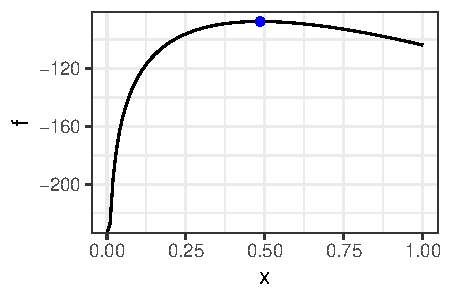
\includegraphics[height=0.35\textwidth, keepaspectratio]{figure_man/ml_poisson_example_2.pdf} 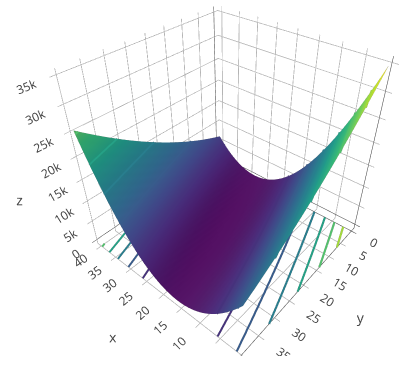
\includegraphics[height=0.35\textwidth, keepaspectratio]{figure_man/ml_linreg_example_3.png} \\
% 	\begin{footnotesize}
% 	Left (Univariate): The log-likelihood of a Poisson distribution. The optimization problem is an univariate optimization problem with $\mathcal{S} = [0, 1]$. Right (Multivariate): The sum of squared errors with regards to the coefficients $(\theta_0, \theta_1)$ of a regression. 
% 	\end{footnotesize}
% \end{center}

% \end{vbframe}

\begin{vbframe}{Note: A Convention in Optimization}

W.l.o.g., we always \textbf{minimize} functions $f$. 

\lz

Maximization results from minimizing $-f$.

\begin{center}
	\begin{footnotesize}
	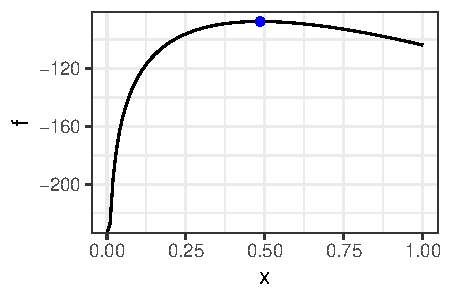
\includegraphics[height=0.3\textwidth, keepaspectratio]{figure_man/ml_poisson_example_2.pdf} 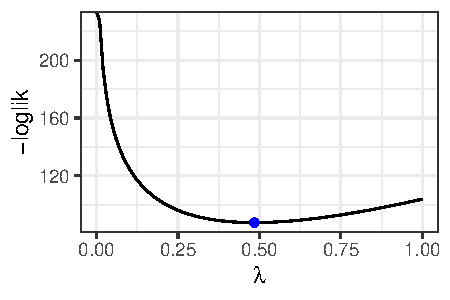
\includegraphics[height=0.3\textwidth, keepaspectratio]{figure_man/ml_poisson_example_3.pdf} \\
	Maximizing the log-likelihood (left) is equivalent to minimizing the negative log-likelihood (right). 
	\end{footnotesize}
\end{center}

\end{vbframe}


\begin{vbframe}{Example 1: Maximum Likelihood}

$\D = \left(\xi[1], ..., \xi[n]\right) \overset{\text{i.i.d.}}{\sim} f(\xv ~|~ \mu, \sigma)$ with $\sigma = 1$: 

$$
	f(\xv ~|~ \mu, \sigma) = \frac{1}{\sqrt{2 \mu \sigma^{2}}}~\exp\left(\frac{-(\xv-\mu)^{2}}{2\sigma^{2}}\right)
$$

\textbf{Goal:} Find $\mu \in \R$ which makes observed data most likely. 

\begin{center}
	\begin{footnotesize}
	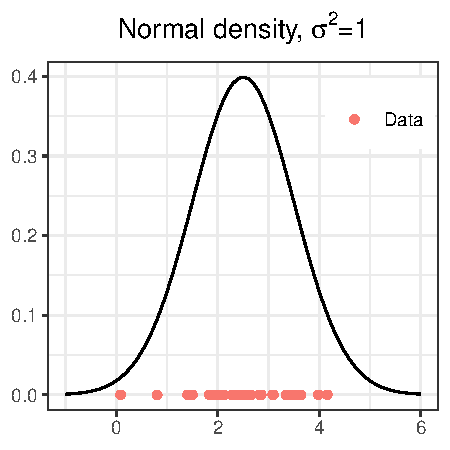
\includegraphics[width=0.4\textwidth, keepaspectratio]{figure_man/ml_normal_example_dnorm.pdf} 
	\end{footnotesize}
\end{center}

\framebreak 

\begin{itemize}
	\item \textbf{Likelihood:} \vspace*{-0.4cm}
 $$\mathcal{L}(\mu~|~\D)= \prod_{i=1}^{n} f\left(\xi~|~\mu, 1\right) = (2\pi)^{-n/2}\exp\left(-\frac{1}{2} \sum_{i=1}^{n} (\xi-\mu)^{2} \right)$$
	\item \textbf{Neg. log-likelihood:} \vspace*{-0.4cm}
$$- \ell(\mu, \D) = - \log \mathcal{L}(\mu~|~\D) = \frac{n}{2} \log(2\pi) + \frac{1}{2} \sum_{i=1}^{n} (\xi-\mu)^{2}$$
\end{itemize}

\vspace*{-0.3cm}

\begin{center}
	\begin{footnotesize}
	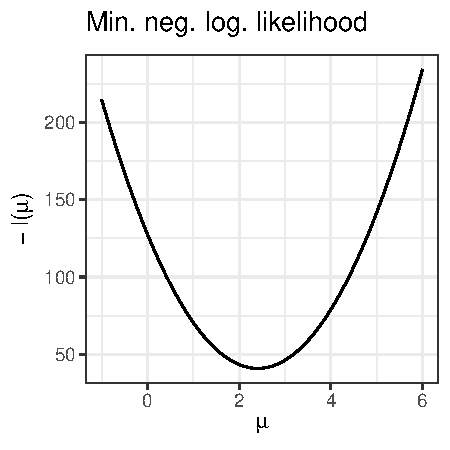
\includegraphics[width=0.4\textwidth, keepaspectratio]{figure_man/ml_normal_example_negloglike_nooptim.pdf} 
	\end{footnotesize}
\end{center}
\framebreak 

$$
	\min_{\mu \in \R} - \ell(\mu, \D).
$$

can be solved analytically (setting the first deriv. to $0$):
\vspace*{-0.5cm}

\begin{footnotesize}
\begin{eqnarray*}
	-\frac{\partial \ell(\mu, \D)}{\partial \mu} = \sumin \left(\xi - \mu\right) &=& 0 \quad \Leftrightarrow \quad \hat \mu = \frac{1}{n} \sumin \xi 
	% \sumin \xi &=& \sumin \mu = n \cdot \mu \\
	% \sumin \xi &=& n \cdot \mu \\
\end{eqnarray*}
\end{footnotesize}

\vspace*{-0.4cm}

\begin{center}
	\begin{footnotesize}
	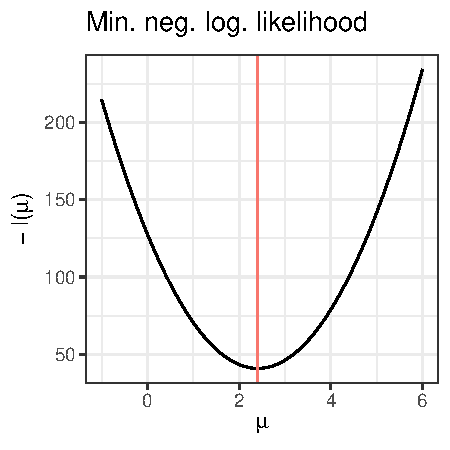
\includegraphics[width=0.4\textwidth, keepaspectratio]{figure_man/ml_normal_example_negloglike.pdf} 
	\end{footnotesize}
\end{center}

\framebreak 

\textbf{Note: } The problem was \textbf{smooth}, \textbf{univariate}, \textbf{unconstrained}, \textbf{convex}. 

\lz 

If we had optimized for $\sigma$ as well 

$$
	\min_{\mu \in \R, \sigma \in \R^+} - \ell(\mu, \D).
$$


(instead of assuming it is known) the problem would have been: 

\begin{itemize}
	\item bivariate (optimize over $(\mu, \sigma)$)
	\item constrained ($\sigma > 0$)
\end{itemize}

$$
	\min_{\mu \in \R, \sigma \in \R^+} - \ell(\mu, \D).
$$

\end{vbframe}


\begin{vbframe}{Example 2: Normal regression}

Assume a dataset $\D = \Dset$ generated according to

$$
\yi = \bm{\theta}^\top \xi + \epsi, \qquad \epsi \overset{iid}{\sim} \mathcal{N}\left(0, 1\right).
$$

\begin{center}
	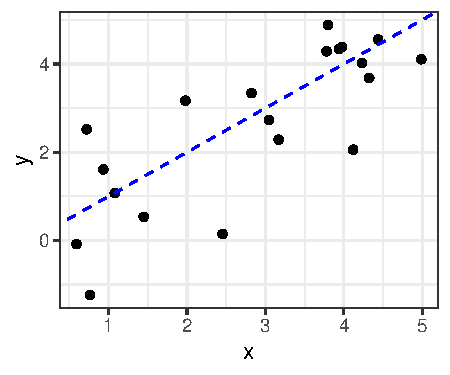
\includegraphics[height=0.4\textwidth, keepaspectratio]{figure_man/ml_linreg_example_1.pdf} 
\end{center}



\end{vbframe}

\begin{vbframe}{Example 2: Normal linear regression} 


In normal linear regression the goal is to find a vector $\thetab$ which minimizes the sum of squared errors (SSE; also: L2-loss): 

$$
\min_{\thetab \in \R^d} \sum_{i = 1}^n \left(\thetab^\top \xi - \yi\right)^2
$$

\begin{center}
	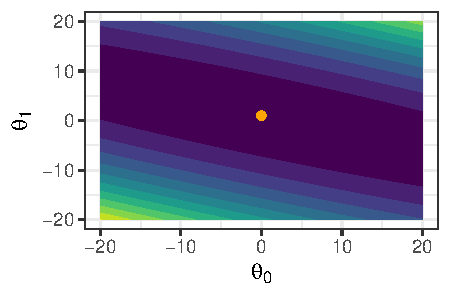
\includegraphics[height=0.30\textwidth, keepaspectratio]{figure_man/ml_linreg_example_2.pdf}
\end{center}

\end{vbframe}

\begin{vbframe}{Example 2: Normal regression}

\begin{center}
	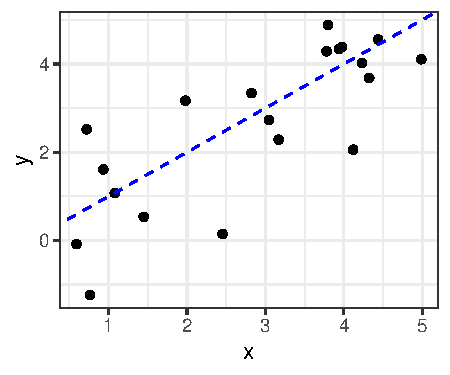
\includegraphics[height=0.30\textwidth, keepaspectratio]{figure_man/ml_linreg_example_1.pdf} ~~ 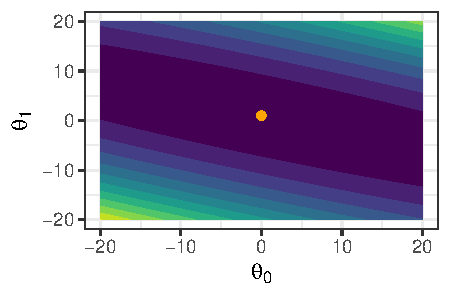
\includegraphics[height=0.30\textwidth, keepaspectratio]{figure_man/ml_linreg_example_2.pdf}
\end{center}

\begin{itemize}
	\item \textbf{Smooth}, \textbf{multivariate}, \textbf{unconstrained}, \textbf{convex} problem
	\item Quadratic form: Obtain a geometric interpretation via Eigenspectrum
	\item The problem has a closed-form solution, which is given by $\thetab = (\Xmat^\top \Xmat)^{-1}\Xmat^\top \bm{y}$, where $\Xmat$ is the design matrix
\end{itemize}

\end{vbframe}

\begin{vbframe}{Risk Minimization in ML}
	
In the above example

$$
\min_{\thetab \in \R^d} \sum_{i = 1}^n \textcolor{violet}{\left(\textcolor{cyan}{\thetab^\top \xi} - \yi\right)^2}
$$

\begin{itemize}
	\item the linear model $\textcolor{cyan}{\thetab^\top \xv}$ by an arbitrary model $\textcolor{cyan}{\fxt}$ % (e.g., something more complex and nonlinear)
	\item the L2-loss $\textcolor{violet}{\left(\fxt - y\right)^2}$ by any loss $\textcolor{violet}{\Lxy}$
\end{itemize}

\lz 

This leads us to \textbf{empirical risk minimization} (ERM)

	$$
	\min \risket = \frac{1}{n} \sumin L\left(\yi, \fxit\right),
	$$

a core concept in machine learning (ML). 

\framebreak 

ML models usually consists of the following components: 

\begin{center}

  \textbf{ML} = $\underbrace{\textbf{Hypothesis Space + Risk + Regularization}}_{\text{Formulating the optimization problem}}$ + $\underbrace{\textbf{Optimization}}_{\text{Solving it}}$ 
  
\end{center}

\lz

\begin{itemize}

  \item \textbf{Hypothesis Space:} Define (and restrict!) what kind of model 
  $f$ can be learned from the data.
  
  \item \textbf{Risk:} Define the risk function $\risket$ that quantifies how well a specific model performs on a given 
  data set via a suitable loss function $L$.
  
  \item \textbf{Optimization:} Solve the resulting optimization problem through optimizing the risk $\risket$ over the hypothesis space.

  \item \textbf{Regularization:} Penalize model complexity 
  
\end{itemize}

\end{vbframe}

\begin{vbframe}{Example 3: Regularized LM}

\begin{footnotesize}

ERM with L2-loss, LM, and quadratic (L2) regularization term: 

\vspace*{-0.2cm}

$$
	\min \risket = \frac{1}{n}\sumin \left(\thetab^\top \xi - \yi\right)^2  + \lambda \cdot \|\thetab\|_2^2 \quad \text{(Ridge regr.)}
$$

\vspace*{-0.1cm}


The problem is still \textbf{multivariate}, \textbf{unconstrained}, \textbf{smooth}, \textbf{convex}.

\vspace*{0.1cm}

ERM with L2-loss, LM, and L1 regularization: 

\vspace*{-0.2cm}

$$
	\min \risket = \frac{1}{n}\sumin \left(\thetab^\top \xi - \yi\right)^2  + \lambda \cdot \|\thetab\|_1 \quad \text{(Lasso regr.)}
$$

\vspace*{-0.1cm}

The problem is still \textbf{multivariate}, \textbf{unconstrained}, \textbf{convex}, but \textcolor{violet}{\textbf{not smooth}}. % The L1 penality is not differentiable if $\exists i$ s.t. $\theta_i = 0$.  

\vspace*{-0.3cm}

\begin{figure}
\begin{center}
	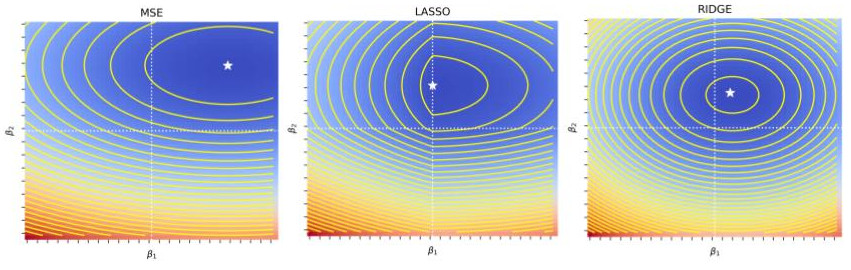
\includegraphics[width=0.8\textwidth]{figure_man/lasso-ridge_medium.jpg}
\end{center}
	\caption{Source: Medium, 2022, Visualize the Loss with Regularization}
	% https://medium.com/@jingwang.physics/visualize-the-loss-with-regularization-2f82666dc0f7
\end{figure}

\end{footnotesize}

\end{vbframe}


\begin{vbframe}{Example 4: SVM}

\begin{footnotesize}
\begin{itemize}
	\item $\D = \left(\left(\xi, \yi\right)\right)_{i = 1, ..., n}$ with $\yi \in \{-1, 1\}$ (classification)
	\item $\fxt \in \R$ scoring classifier: Predict $1$ if $\fxt > 0$ and $-1$ otherwise. 
\end{itemize}
\end{footnotesize}

ERM with LM, Hinge loss, and L2 regularization: 

$$
	\min_{\thetab} ~\sumin \max\left(1 - \yi f^{(i)}, 0\right) + \lambda \thetab^\top \thetab, \quad f^{(i)} := \thetab^\top \xi
$$

\vspace*{-0.2cm}

\begin{columns}[T] % align columns
	\begin{column}{.58\textwidth}
		\begin{center}
			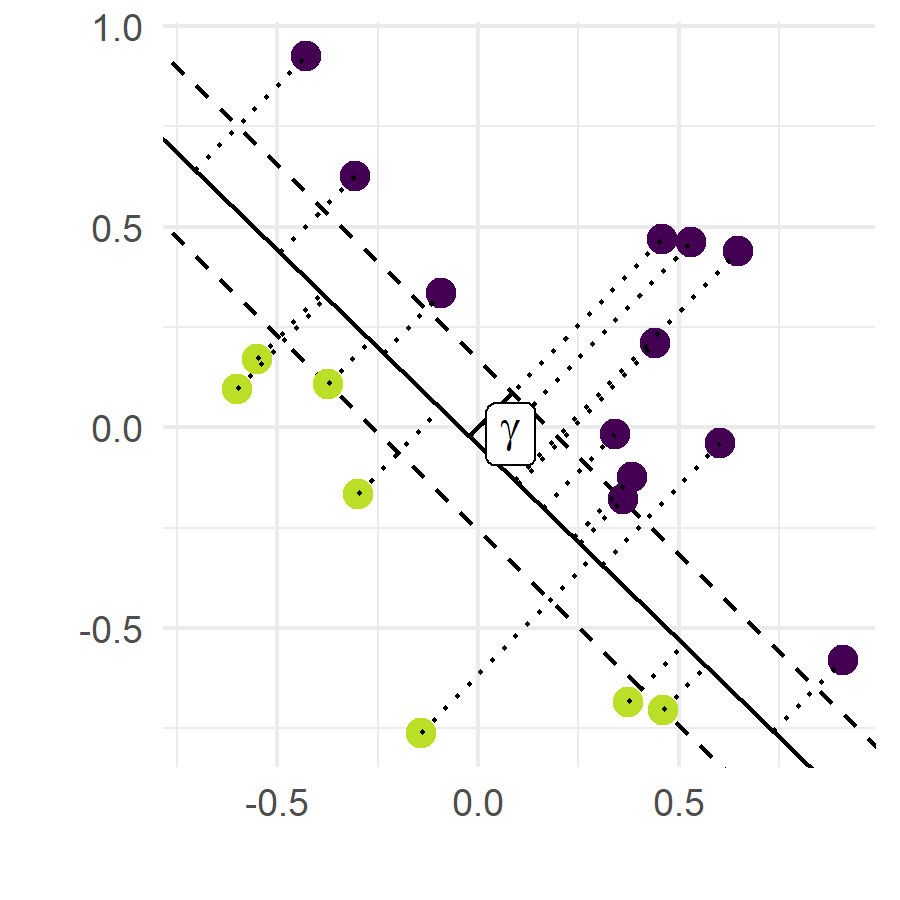
\includegraphics[width=0.6\textwidth]{figure_man/svm_geometry.png} 
		\end{center}
	\end{column}
	\begin{column}{.38\textwidth} \vspace*{1.5cm}
		\begin{footnotesize}
		This is one formulation of the \textbf{linear support vector machine}. The problem is still \textbf{multivariate}, \textbf{unconstrained}, \textbf{convex}, but \textcolor{violet}{\textbf{not smooth}}.  
		\end{footnotesize}
	\end{column}
\end{columns}

\framebreak 

Understanding Hinge loss $\Lxy = \max\left(1 - y\cdot f, 0\right)$

\begin{footnotesize}
\begin{center}
\begin{tabular}{ c | c | c | c | c }
$\mathbf{y}$ & $\fx$ &  \textbf{Correct pred.?}  & $\Lxy$ & \textbf{Reason for costs}  \\ \hline
 $1$ & $(- \infty, 0)$  & N & $(1, \infty)$ & Misclassification \\
 $- 1$ & $(0, \infty)$ & N  & $(1, \infty)$ &  Misclassification \\
 $1$ & $(0, 1)$ & Y & $(0, 1)$ & Low confidence / margin \\
 $- 1$ & $(-1, 0)$  & Y  & $(0, 1)$& Low confidence / margin\\
 $1$ & $(1, \infty)$ &  Y & $0$ & -- \\
 $- 1$ & $(- \infty, -1)$ &  Y & $0$ & -- \\
\end{tabular}
\end{center}
\end{footnotesize}

\vspace*{-0.3cm}
\begin{figure}
	\begin{center}
		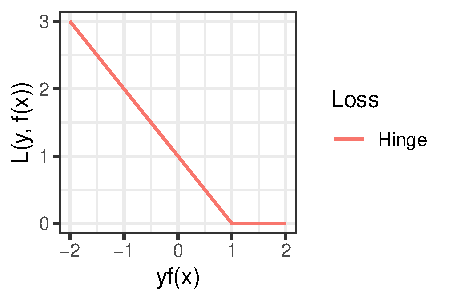
\includegraphics[width=0.5\textwidth]{figure_man/hinge.pdf}
	\end{center}
	% See hinge_vs_l2.R
\end{figure}

\framebreak 

\textbf{Kernelized} formulation of the SVM for nonlinear $f$: 

\begin{eqnarray*}
	\min_{\thetab}\sumin L\left(\yi, \bm{K}_i ~\thetab\right) + \lambda \thetab^\top \bm{K} \thetab 
\end{eqnarray*}

with $k(\xi, \xi[j])$ positive definite kernel function, and $\bm{K}_{ij} := k(\xi, \xi[j])$, $i, j = 1, ..., n$ kernel matrix, $\bm{K}_i$ is the $i$-th column of the kernel matrix. 

\vspace*{0.2cm}

\begin{columns}[T] % align columns
	\begin{column}{.38\textwidth} 
        Kernelization 
        
        \begin{itemize}
        	\item allows introducing nonlinearity
        	\item without changing characteristics of the optimization problem (convexity!)
        \end{itemize}
	\end{column}
	\begin{column}{.58\textwidth}
		\begin{center}
		    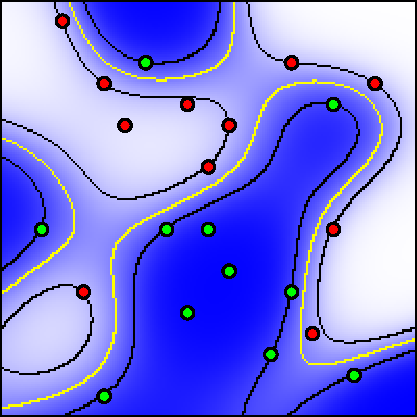
\includegraphics[width=0.4\textwidth]{slides/02-optimization-problems/figure_man/nonlinear-svm-c.pdf}
		    % https://github.com/slds-lmu/lecture_i2ml/blob/master/slides/nonlinear-svm/figure_man/kernels/nonlinear-svm-c.pdf
		\end{center}
	\end{column}

\end{columns}





\end{vbframe}


\begin{vbframe}{Example 5: Neural network}

The (computational) complexity of the optimization problem 

$$
\text{arg} \min_{\thetab} \risket,
$$

(i.e. smoothness, convexity) is influenced by model structure and loss. 		
\vspace*{-0.3cm}
\begin{center}
		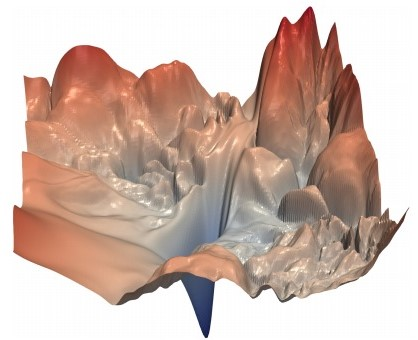
\includegraphics[width=0.3\textwidth]{figure_man/ml_landscape.jpg} ~~~ 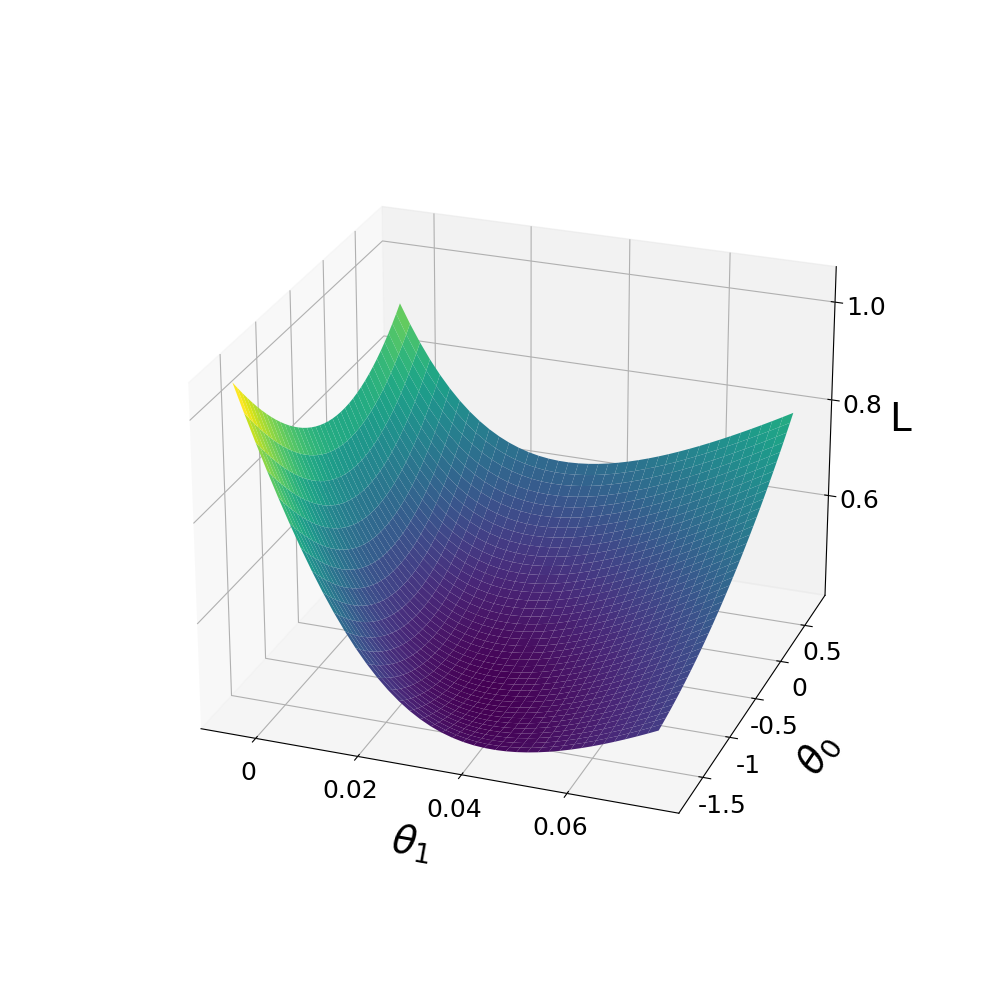
\includegraphics[width=0.3\textwidth]{figure_man/log_reg.png}
	\begin{footnotesize}
		\newline
		Loss landscapes of ML problems. \\ Left: Deep learning model ResNet-56, right: Logistic regression with cross-entropy loss
		\newline
		Source: \url{https://arxiv.org/pdf/1712.09913.pdf}
	\end{footnotesize}
\end{center}	

\end{vbframe}


\endlecture

\end{document}
